
\chapter{Identity}

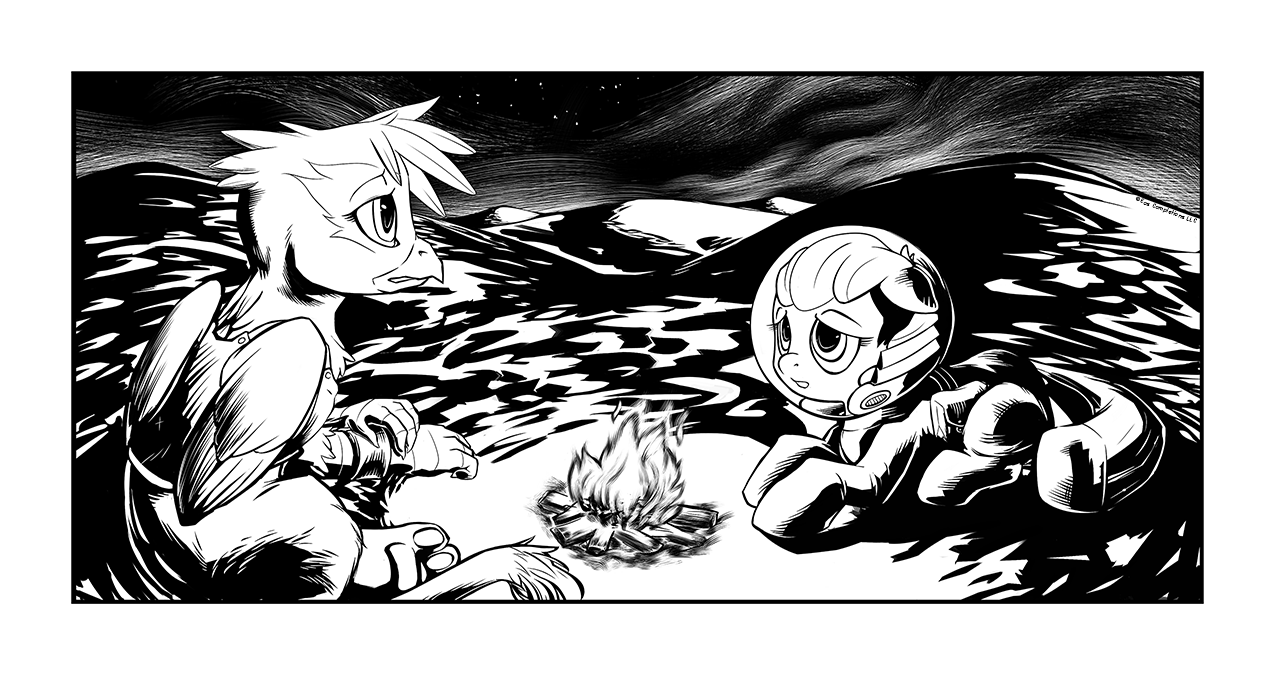
\includegraphics[width=0.9\linewidth]{image10.png}

\begin{intro}
In the desert you can remember your name,

'cause there ain't no one to give you pain.
\end{intro}


\englishdaytimeplace{9}{2:00 A.M.}{Sun City Downtown, Big 52 SC Branch}

``Fuck this headache, I can't sleep.'' Henrietta rubbed her sorry head. Puppy was a good aim, and had a fair bit of strength when it came to throwing things. Now Henri was feeling the full force of Puppy's skill. The day had been a hard one with a lot of work, dismantling the buildings in the outer belt and bringing the materials to the residential area. If she hadn't had that wound, she would have been asleep like everyone else.

``Next time I see that yellow devil, I'm going to spank her so bad that her rump could be used as a landing signal on foggy nights.'' By the way, what was she doing in Sun City? The whole place was a trap, with that hypnotic buzz that could bend your will and---

Henri's eyes widened in sudden realization as she muttered to herself, ``Wait a single eggfucking second\dots The buzz is gone. The damn buzz is gone, and I can think clearly! I've got to get out of here!'' She stood up, spreading her wings, ready to take flight, but froze in place as soon as she noticed the other griffons. There were five of them in the room. Two were the Talons that she tried to lose by diving into this fucking place, while the other three had the Talons tattoos, but wore no armor and didn't appear to be armed.

``At last, it's payback time!'' A cruel grin appeared on Henri's beak as she unsheathed her bowie knife and stepped toward the first sleeping griffon. She was one of the unarmored ones, sleeping intently because of the day's hard work. The young half-eagle moved slowly and silently, like a serpent in the grass. She approached her victim from behind, ready to grasp her beak and slit her throat. Very slowly she leaned over her victim's head and\dots noticed the eggs.

``Oh fuck no.'' The fire in Henrietta's eyes died as she looked at the two eggs that the griffon was hugging in her sleep. Rage became hesitation and her resolve shattered. Killing a mother in her sleep was beyond any hunger for revenge she had. But the other four, on the other claw\dots

The other four what? Two were just victims of the place, and one of them could have been the father of those eggs. Besides, they were totally unarmed and possibly didn't have anything against her. And the two that chased her inside Sun City were sleeping hard enough that she was going to be miles away before they realized that she was gone. What was the point in killing them like this?

``I'm not a backstabber.'' Henrietta turned on her tail and headed for the door, but stopped as she noticed a spot of pink in a corner of the room. Willy Fail, Stinky Mail, or something like that. Puppy's doll. Hell, she had almost forgotten about the doll. ``Oh fuck, Puppy!'' Stupid feather head, she had almost forgotten about Puppy!


\horizonline

\englishdaytimeplace{9}{2:30 A.M.}{Sun City Downtown, Big 52 SC Branch}

Sitting in the red shadows of the control room, Puppy was still confused. She had no idea who that mare that visited her before Mister Voice came back could be, and she wasn't sure if the newcomer was a pretty pony. Even thinking about that scary mare talking in her head was enough to send shivers down her spine. She hoped that she wasn't going to return any time soon.

Luckily enough, Puppy was now in good company again. Whatever problems the mare's voice had created were far enough away to let Puppy think about more pressing matters. First things first, she needed to find her a name, since Miss Voice was already taken.

``Ah, she's a she, so miss is okay, and she is, ah, scary? Scary Voice? Sounds wrong\dots'' Puppy frowned. This was going to be a hard nut to crack. ``Head Voice? Meh. Nightmare Voice? Too long\dots I know! Creepy Voice, because she is creepy! Yay!''

The HUD on the helmet tinged, informing Puppy that the mission ``Shaping Nightmares'' was successfully accomplished. Yes, she was good. No challenge could slow her, not even coming up with names for things. Okay, maybe something long to read could still be a mighty foe, and counting things that were more than her hooves was hard, and even opening pickle jars, that had always been an impossible feat\dots But everything else was easy, right? Go Puppy!

Now that the cheering was done, it was time to undertake part two of her master plan, finding Henri and getting out of here as quick as a pony at the Running of the Leaves. ``Okie dokie, Mister Voice, where's Henri?''

{\mt ``Henrietta Firebright set as primary target.''}

The arrow on the compass integrated in Puppy's helmet disappeared and reappeared pointing to her left, displaying a distance in meters that rapidly diminished until it reached a single digit.

``Yay! It's adventure ti---''

\emph{BLAM!}

\emph{CRASH!}

\emph{BLAM!}

One of the windows exploded, and with a flutter of wings a young griffon wielding a pair of .45 pistols blitzed inside the room through a cloud of glass and bullets. ``Hold on, Puppy, I'm here!'' She tumbled across the floor trying to identify any possible hostile target, fired twice at the lights in the ceiling, which plunged the room into darkness, and jumped behind a desk before upturning it to use as an improvised barrier, all in the space of just a few seconds.

A smile grew across Puppy's muzzle as she watched the show. Wow, this was so cool! Henri was totally the best pony! She was like that griffon in that movie, Liòn: the Professional. She stomped her hooves on the floor, cheering her friend's performance. ``Woohoo! Go Henri, you rock! Way to go!'' A couple of bullets narrowly missed Puppy's helmet before Henri recognized her friend.

``Lie flat on the floor Puppy, I'm taking care of them! Leave this little pony alone, you brain eaters!''

``Wut?'' Puppy tilted her head with a curious expression.

Noticing that nopony was firing back and that there was no movement in the room, a thought suddenly struck her. Could it be that Puppy wasn't actually in danger? Henrietta smiled in embarrassment as she stopped acting like a special forces pony and took a decent look around. Putting away her guns, she stroked back the feathers on her forehead and assumed a cool demeanor. ``Hey, Puppy, still all in one piece?''

She checked her legs and tail, then smiled and nodded to her friend. ``Yup, I forgot nothing! Is Silky Tail all right?''

``Your doll? Sure, want it back?'' Henrietta grabbed the pink plushie and waved it. Puppy shook her head.

``Nopey mopey, she is fine with you. I asked her to keep an eye on you and she warned me that you were in danger, so I came here but at the beginning you were all grumpy and scolded me then you flied away and didn't want to talk with me anymore, so I waited for the night because I had this super duper mega plan but before I had to say to the mayor that his town was ugly but then the mayor wasn't a mayor, but a stoopid voice that told me bad things, but I was smarter and he said he was sorry and now he's gone away, so I'm smarter than Blue Voice.''

Henrietta rose a claw. ``Wait wait wait! I see you moving your muzzle, but all I hear is blah blah blah. None of it makes sense and we're in a hurry. Everyone is sleeping right now, but very soon someone will wake up and realize that the buzz is gone. This place is filled with Enclave pegasi, Talon griffons, and ponies from at least two different tribes, and they are all sitting on a fortified source of pure water and fresh food.''

Puppy tilted her head in confusion. ``Uh, okie dokie?''

Henri facepalmed. ``All right, simple version. In a couple of hours Tranquility Lane will become War Zone: Sun City, and we have to get our tails out of here before that happens, capeesh?''

``War zone? Like when ponies are mean with each other?'' Puppy asked with some degree of doubt.

``Yes, exactly. Each group will want to take this place for themselves. Now, leave behind everything heavy you have in your bags because we need to get out of here, and fast.''

Puppy frowned. ``But why do they have to argue? Ponies are pretty and nice. They shouldn't be mean!'' She explained her theory about pony behavior as if it was something so simple that it was impossible for it to be some other way.

Henrietta opened her beak to reply that an entire world had turned into a wasteland as a legacy of pony kindness, but trying to explain such a concept to Puppy was harder than teaching an anvil how to swim. And even more importantly, it required time that they didn't have. ``Yeah, exactly, but we have to go away right now anyway, because you have to find your mom, right?''

Puppy nodded vigorously. ``Yush! I have to go to a peggysus fly place named Blue Idontknow, but Miss Happy told me that now it's called Something Manner. Ah, I don't remember the name very well, but there's an arrow on the compass so I can't miss it!''

Henrietta sighed. ``Let me guess, it's south.'' She pointed a direction with her claw.

Puppy stared in surprise at her friend. ``Woah, how did you know that? Are you a wizard?''

``Yeah, sure, I'm the best magician in Equestria. The Great and Powerful Henri. Now please dump everything you don't need or we won't be able to fly.'' Henri paused for a moment, noticing something new in her friend. ``Say, how long have you had a blue streak in your mane?''

A thin line of blue ran through Puppy's blonde mane, starting from her forehead just above her right eye and ending at three quarters down her neck. The line was made of a couple shades of blue, in a similar way to that mare from the Ministry of Magic, Twilight Snarkle or something like that.


\horizonline

\englishdaytimeplace{9}{3:00 A.M.}{Sun City Downtown, Big 52 SC Branch}

Puppy risked opening one eye and looked down. The world rushed away from her into the night. Large skyscrapers zipped past below her, and dark, deserted roads trailed off into the distance under her nose. Much too far under her nose to be comfortable with.

``ARE WE THERE YET?'' She grabbed Henrietta's neck tight enough to choke her.

``Ack! Loosen those hooves, pony, you're going to make both of us crash!'' At first it just seemed natural to Henri to fly away with Puppy. She was really small and, once she threw away all those useless scraps, she was lighter than a military backpack. Problems came when Puppy discovered that she hated flying. ``Just close your eyes and pretend you're having a regular piggyback ride or sing something!''

Puppy already had her eyes sealed tighter than a Stable door, but it didn't seem to help at all.  Seeing all the houses from above and seeing the roofs run and run away in a crazy stream of colors already scared her enough. This wasn't like looking down from a tower. Towers didn't go around, and they had floors! She liked floors, they were so\dots so flat, and floory! ``Please please please I will behave! Put me down pleeeease!''

``Oh c'mon, are you a scaredy pony? Have some faith in your friends!'' With a stroke of her wings, Henrietta gained a little altitude, flying between two skyscrapers and soaring past downtown, high above the residential area of Sun City. The fresh night air tasted of dust and old, but the south winds carried a new scent, the sea. ``Just relax and enjoy the trip. Sing something!''

Singing something. Yes, that always helped Puppy. She just had to sing a song and everything would be better! She cleared her throat and tried singing the first thing that came to her mind.

``
\begin{song}
	Humpty Dumpty sat on a wall
	
	Humpty dumpty had a great
\end{song}
OH PLEASEPLEASE\emph{PLEASE}\/ PUT ME DOWN NAO!''

She was dancing the pony pokey on Henri's back, but a griffon's constitution is one of a predator, happy to fly with an adult pony struggling in her claws and still capable of gaining altitude in the meantime. ``Stop it, I'm not letting you fall! Yeow! Don't pluck me! Have you the slightest idea of how long those plumes take to grow back!?'' Sick of being pestered by the panicking pony, Henri bumped Puppysmiles off her back and caught the falling filly with her talons. ``All right, at least this way you don't risk falling! Hold on, we'll land as soon as we're out of the ruins!''

``EEEEEEP!''

``Don't wet your suit! It's a couple kilometers at most, so we gotta put some distance between us and this place before it blows up!'' She accelerated, pushing herself harder so that the trip would be as short as possible, but carrying a howling banshee in the night sky was going to wake some sleeping ponies. Henrietta could only pray to her lucky star that nopony would poke their head out a window and look for the source, or that they wouldn't care enough to bother.


\horizonline

\englishdaytimeplace{9}{3:30 A.M.}{Serpent Desert, Big 52 SC Branch}

``I wasn't scared at all, you know. I was just, ah, cautious. I mean, with all those roofs looking the same and the wind you could, ah, lose yourself, and it's much better seeing the names of the streets when you don't know where you are going.'' Now that she had all of her hooves on solid ground again, Puppy was desperately trying to regain her macho appeal, but the effort was a little wasted by Henrietta literally rolling on the road laughing.

``Priceless! You're priceless, Puppy!'' She gasped as she tried to inhale, wiped a tear from her eye, and burst into another laugh. ``How did you scream? \emph{Eeeep!}\/ Do it again, do it again please!''

Puppy pouted, sat down and sighed. ``Hey, I wasn't the one that got lost in a city! I've seen chickens smarter than y---'' 

\emph{BLAM!}

Puppy looked down at the hole in her suit, right where her heart should be. ``Hey! There are already enough bullybots doing that!''

Henrietta got up and waved her gun in a dismissive manner. She still hadn't stopped smiling, even after she shot Puppy. ``Aw, don't complain. You got torn apart by a manticore and you're still standing! How could you get hurt by a bullet or two?'' 

\emph{BLAM!}

\emph{BLAM!}

Another couple of shots pierced Puppy, once in a leg and again in her chest. ``Stop it! This stoopid suit starts saying absurdities and mumbo-jumbos every time this happens!'' A thin thread of pink poured from the holes made by the griffon's gun.

``Okay, okay, but you stop calling me a chicken.'' Henrietta yawned and put away her pistols. ``Just for your information, normal ponies die when they are shot, even ghouls, so don't try this on other ponies, okay?''

Puppy nodded, a bit confused, then tilted her head. ``But I am a normal pony!''

``Hey, hey, I didn't say otherwise\dots Woah, are we a little upset today? Want me to sing you a lullaby?'' Henri asked with a mocking tone.

Puppy nodded vigorously. ``Sure! I lovelovelove lullabies! Can we sing \emph{Hush now quiet now}\/?''

Henri facepalmed. What was the point of trying to provoke this foal if she couldn't even tell when she was being mocked? ``You're a lost cause, Puppy. ''

\begin{song}
		``Hush now, quiet now, it's time to lay your sleepy head!
	
		Hush now, quiet now, it's time to go to beeed!''
\end{song}

Henri sighed and started walking south. ``Why, dad, why do I owe my life to this idiot twice?'' She smiled and turned her head toward Puppy. ``Hey, jump on your red racer, and I'll fly above you. We have a lot of ground to cover if you want to get to Rust Manor by tomorrow.''


\horizonline

\englishdaytimeplace{9}{10:30 P.M.}{Serpent Desert, Big 52 SC Branch}

A small campfire cast the shadows of Puppy and Henrietta over the sand dunes. The two travelers were sitting next to the little source of light and heat. Henri was eating something from a tin can, but from the faces she made it wasn't exactly griffon food. The clouds above the desert helped the place to maintain its temperature even during the night.

``So, Puppy, this Blue Voice told you that you're a robot?'' Henri's expression was hard to read, like she was trying to keep a poker face until she finished telling the whole story.

``Yes, and he seemed double super sure of this. I almost fell for it too, but then arrived Creepy Voice that told me that it was impossible because, ah, I didn't understand that part, but it seemed quite okay when she said it.'' Puppy nodded wisely, as if this was everything that she needed to know.

Henri shrugged. ``So, a computer tells you that you're some sort of crazy machine, but a hallucination says otherwise. I think you just got dazed by the EMP grenade because of the backlash on your suit's circuitry and you had a dream.'' Henrietta yawned before continuing. ``But I don't think you're a robot, Puppy. Robots explode when shot, and, besides, robots are intelligent.''

Puppy frowned. ``So, what do you think I am?''

Henri stretched her hind legs and took a seat on her improvised couch. ``You? You're bad news, that's all I need to know. But I like you, so you can hang with me and be cool like big sis Henri.''

Puppy trotted over to her companion and met Henrietta's gaze. Her eyes were two large glowing pink lights in the darkness of the night. ``Yes, but, I am a pony, right? I mean, it doesn't matter if I don't eat or drink or never need to potty, right? I'm a pony\dots''

\emph{She seems worried, this robot thing is actually scaring her\dots Oh, fuck, why me?}\/ Henri was completely exhausted, and she didn't need a foal with an existential crisis at the moment. All that she wanted was to get some sleep. She patted Puppy on the helmet, yawning. ``You can be whatever you want, Puppy. You are a good pony, and good ponies are the most rare variety in Equestria nowadays. As long as you think that you should be a pony, then you'll be a pony. Now go to sleep, please.''

Puppy smiled and tried nudging Henri through her helmet. ``Thank you Henri, you are my very best chicken friend!'' Crouching next to Henri, she sighed and waited, since she wasn't sleepy at all.

\dots

\dots

``HEY! What did you mean by I'm not a robot because they are intelligent?'' Puppy poked Henri in a flank, but Henri just snickered and turned on her other side.

``Priceless.''

Puppy kept whining and poking her friend to try and make her talk, but Henri began to snore loudly, leaving a frustrated Puppy complaining in front of a dying fire.


\horizonline

\englishdaytimeplace{10}{1:00 A.M.}{Serpent Desert, Big 52 SC Branch}

It was still dark and Puppy couldn't sleep. She wasn't tired at all, but Henri didn't want to be disturbed, so Puppy did the most logical thing she could think of: sightseeing the desert by night, because wise Puppy is wise.

So far this place had deluded a lot of Puppy's expectations. After all those movies with the cowponies and the buffaloes, she was quite sure that a desert should be crowded with so many skulls, arrows, tents, and other things that you couldn't even find a place to put down your hooves. But after spending a few days in the ``real'' desert, she had the slightest suspicion that all the buffaloes must have gone away for some sort of holiday. She at least hoped to find a lizard in a place called Serpent Desert, but all she had seen so far were a couple of carts half buried in the sand, and a large parasprite with long teeth that was building something similar to a nest. When she approached it, the parasprite flew away, avoiding her.

{\mt ``Warning. Hostile detected. Analyzing: Mutated parasprite, Parador variety. Threat level: deadly.''}

``Aw, why is every pretty fluffy animal in this place so shy? I just want to make friends!'' said the two-hundred-year-old monster to the mutated, murderous offspring of Mother Nature and Father Taint.

``Hey, Puppy, it's been a while. You travel a lot, don't you?'' said a staticky voice, interrupting the little exploration of miss adventure. She smiled broadly and turned to her friend.

``Mister Questioner! Where have you been?''

``It's Watcher. I watch things, Watcher?''

Puppy nodded, still smiling. ``Okie dokie, Mister Questioner, can I watch things too?''

From the speakers of the spritebot came a soft and metallic chuckle. ``Puppy, Puppy never changes. How are you? I've heard that you had a little adventure in Tunnel Town, and now I find you south of Sun City.''

``Yush! I met a lot of nice and pretty ponies! There was this chicken called Henri, and then Asso and Sweet Flower, Happy, Jamie, and a lot of other friends!''

``Wow, you are quite lucky to have so many friends, aren't you? And say, have you been in Sun City?'' The voice was trying hard to maintain a neutral tone, but it seemed very curious.

Puppy frowned. ``Yeah, it was like a super duper box with streamers and mighty fine wrappings, but with oatmeal inside. Everypony was grumpy, they didn't want to talk with me or to play with me, and their mayor was a stoopid voice that told me bad things.''

``Bad things like what? Would you like to talk about that?'' Watcher's voice betrayed a hint of worry.

Puppy looked away. ``He told me that I wasn't a pony, but a robot, then I used that big teapot that puts robots to sleep, and I was hit too. Everypony keeps telling me that I am no robot, but why I---''

``Tut, tut, Puppy. Don't fret your little head. If there's something that I'm completely sure of, it's that you're not a robot. That voice probably read some data from a sensor scanning you, but it was a machine and couldn't see beyond your appearance. You are a pretty pony, okay? Now smile and show me that everything is all right.''

Puppy nodded and smiled a little.

``Very well. Now, zombie ponies in a nice city. Did you find anything like a buzz or a humming sound all over the place?''

``Nopey mopey, but Henri told me that the buzz was gone and that all the pretty ponies were going to wake up and start being not-so-pretty.''

``Oh, so at last the interference is gone. I can finally take a look inside the place then. Let me guess, you stopped it?''

Puppy frowned. ``No, I just went there because I was told that Henri was in danger, but she wasn't! She just acted like a stoopid chicken flying around and not paying attention to me, like every other pony in the town, so I went to this Blue Voice Mayor and we had this big argument. He wanted to be smarter than me, so I took the blue teapot and---''

``Ah, excuse me, what is this blue teapot?''

She sighed, helmethoofing. ``Why I have to explain everything to everypony? It's a teapot, round and shiny with a blue pointy head. I found it inside a rusted cart in that place in the swamp.''

``All right, so you detonated an EMP shock shell in front of a supercomputer. Yes, you stopped the interference. And what about the new look?''

Puppy tilted her head, trying to look at her mane. ``You mean the blue line? I don't know, it appeared when I woke up the other day after speaking with Cre---''

``Hey Puppy, who's there? Hold on, I'm coming!'' Henrietta's voice interrupted the little pony.

``Sorry little one, I've got to go. You can tell me this story another time!'' Without even waiting for an answer, the spritebot made a noise like static and began playing some patriotic music.

Henri quickly vaulted over the top of the dune separating her and Puppy, checking the surroundings with a gun in both her talons. As soon as she decided that there was no immediate danger, she put away the weapons and scolded Puppy. ``Bad pony! Stop playing around with the spritebots and come back to the camp!''

Puppy waved a hoof at the floating robot as if left and trotted back to her feathery friend. ``I wasn't playing, I was telling him my interesting adventures!''

``Yeah, sure. Now let's get back to sleep. Tomorrow will be a long day.'' She rubbed Puppy on the helmet and they went back to their camp.

Half an hour later, a scared parador could finally go back to building its nest in peace.


\horizonline


{\rt
Good morning fillies and gentlecolts! This is Lonesome Pony, and you're listening to Radio 52! Find a radio better than us, and I'll personally give you a treat! Who, DJ PON-3? Please, I've heard he's a she! Really! And during clear nights she transforms herself into a giant three headed diamond dog! No kidding, just go to Tenpony tower during a clear night and you'll see! ``But L.P., There hasn't been a clear night or day since the spells fell!'' Not my problem, my little ponies! You just stay tuned on Radio 52 and stop blabbering about crossdressing radio DJs!

Now, back to work. It's news time! Yesterday morning, Sun City woke up from a nineteen year long sleep. I don't have any details, but it seems that during the night somepony assaulted the central tower of the town, stopping whatever device was controlling the minds of everypony in the city! Yes my little ponies, you heard me correctly! Nopony ever came back from Sun City because the whole place was under the effect of a giant mind control device! This is crazy!

And guess what the pretty residents did the very same moment they realized that the mind control was gone? You guessed it! They started fighting each other for control of the town! If you are going to cross Serpent Desert, take a long detour, following Green Route East or take the Chasm Trail, but stay away from Sun City until things settle down! I repeat, stay away from Sun City and avoid Red Route if possible.

Now, for the ones who like a little gossip, who's responsible for the change of administration in the city? Do I really need to say the name? Yes my little ponies, our little resident hero saved you from a never ending sleep so that you could freely and willingly WASTE YOUR LIVES KILLING EACH OTHER! Don't you even feel ashamed? I\dots I don't want to talk about this. Take some music while I look for answers in an empty bottle.

What we've got here is a failure to communicate. Some ponies you just can't reach\dots
}

The voice of the DJ was replaced by music.

\begin{music}
		Look at you young colts fighting.
	
		Look at your fillies crying.
	
		Look at your young colts dying,
	
		The way they've always done before.
\end{music}

\horizonline

\englishdaytimeplace{10}{10:30 A.M.}{Rust Manor, Big 52 SC Branch}

Rust Manor seemed like exactly what it said on the tin: a large, reinforced barricade made up of huge air wagon carcasses forming a ring a hundred meters in diameter around what was originally the offspring of a bunker and an air traffic control tower. The whole structure was once coated in thick, reinforced steel plates, but now all the metal was rusted, and the large tower seemed a monument to the concept of neglect itself. Nonetheless, the little town was a lively trading post, with several caravans stationed outside of the northern gates, and half a dozen town guards scanning the surroundings from a crown of guard towers built on top of the wall.

Henrietta called after Puppy, trying to get her to stop when they were a couple of kilometers from the town, where the low hills became a flat plain peppered with craters. During the war the airfield was heavily attacked with conventional weapons, flattening every structure except the fortified control tower. The open terrain gave a sniper a long line of sight, which made it easy to take care of any possible nuisance. 

``Wait for me, red bolt!'' Henri landed in front of Puppy, making her stop and kick up a cloud of dust.

``Woah, look where you are landing! I was running there before you!''

``Yeah, sure, whatever. I need you to listen carefully, fishbowl head. I have to leave you again, but this place is safe, so you won't find troubles.''

Puppy's eyes grew large and teary while she was already starting to pout. ``But-but why? I don't want you to go away!''

``Yeah, I know. I'm cool, and without me you are quite clueless, but those guys that were after me in Sun City had a whole day behind their wings. It's possible that they're waiting for me here. I don't want you to get involved in my troubles.''

``Ah, if the bad chickens are after you we can explain to them that you are a good girl, and you will behave and say that you are sorry for whatever you did so they will let you be, can we?''

Henrietta sighed, patting Puppy on the helmet. ``The story is a little more complicated than that, involving things like me having shot a couple of theirs and them wanting my head, so\dots No, I don't think we can just say that we are sorry, especially since I'm not sorry. They killed my father.''

``Oh,'' Puppy lowered her eyes, trying hard to think of something else. ``But you can't just bully those that bully you! I mean, they're not bullybots, they're pretty kitties! You can't bully kitties!''

Henrietta snickered. ``Yeah, pretty kitties. That's why I'm not going into town. If I avoid them, there will be no need for me to kick their sorry butts, and they won't be able to bully me.'' Henri shrugged. ``And that ends the topic. Take care Puppy, I'm sure we'll meet again.'' Without even waiting for a reply, Henrietta jumped into the air, and with a couple of strokes from her wings she was already out of range of the eventual stone throw from Puppy.

Puppy galloped after her friend for a few hundred meters, calling desperately for her before stopping and sighing. ``Aw, this is not fair. She didn't even hug me goodbye!'' She raised her head to the sky, screaming, ``Silky Tail, take care of her! She's in your hooves nao!''


\horizonline

\englishdaytimeplace{10}{11:00 A.M.}{Rust Manor, Big 52 SC Branch}

The sniper had been keeping the yellow dot in her sight since she had come over the last hill, but the unicorn mare was uncertain of what she was looking at. The guard put a hoof on an interphone. ``Last Stand here, I have a contact at one, one, eight, six, south. It seems to be a pony in a yellow suit, could be that ghost from the radio, fits the description pretty well. Are ghosts welcome here?''

The speaker replied in a storm of statics and electric whistles. ``Keep an eye on the target and see what it does. Call again if you notice any hostile behavior, otherwise let it approach the gates.''

``Roger, roger.'' The mare went back to her position.

In the meantime, Puppy reached the first caravans, drawing the attention of almost every hired guard in the area outside the walls. A lot of ponies were whispering to each other, and a couple of them reached for their weapons. She didn't even notice their reactions. Her mother was somewhere inside the big town, and this was all that she needed to know. ``Hi, I'm Puppysmiles! Have you seen my mom? Mister Voice told me she is here!''

All the ponies in the area looked at her, then one of them sighed. ``Oh, it's just Lonesome's Ghost.'' The guards put away their weapons and a couple of merchants that stopped chatting at Puppy's appearance went back to their business, but nopony replied to her question.

``Uh, I guess that's a no?'' She was confused. Her status changed from center of attention to completely ignored. This couldn't be right. ``Aw, when you want something done, you have to do it yourself. Okie dokie, Mister Voice, where now?''

{\mt ``Analyzing. Loading local maps: Blue Feathers Airfield. Matching failed. Loading backup data. Finding points of interest. Points located: one---Control Tower. Control Tower set as next way point.''}

The arrow moved on the compass.

``Oh, inside the town, all right!'' Puppy trotted merrily towards the gates, but was stopped almost immediately by an old stallion wearing mercenary armor and a dusty hat. Somehow the eyes of this pony held something familiar, as if the little pony had seen them somewhere before.

\rcpr{``Hey mom, why that pony has only three legs?''}

\rcpr{``He's a war hero, Puppy, please don't bother him. He's very tired.''}

\rcpr{``Yeah, tired of giving my leg for a fucking useless war against fucking enemies I don't even care about because of a fucking goddess that puts a bunch of coal in front of a pony's life!''}

\rcpr{``Tee-hee, the pretty pony says strange words!''}

\rcpr{``No Puppy! Forget that word, it's a bad word! And you, you should be ashamed of using such a language in front of a foal!''}

\rcpr{``Fuck off, bitch.''}

\rcpr{``Let's go away, Puppy, come with me.''}

\rcpr{``But Mom, I wanted to---''}

\rcpr{``Yeah, pink rat, trot after your mom! There's nothing to see here\dots''}

Puppy blinked, lost in her memories. When she came back from her personal world, the old pony with the angry eyes was still standing there, so she stared back at him and tilted her head. ``Hi, have you seen my mom?''

The mercenary spat on the ground. ``Are you deaf or what?''

Puppy sat down, looking confusedly at her interlocutor. ``Ah, sorry I didn't hear the question. Why are you angry? Did I do something wrong?''

The pony snickered. ``I asked you if you think you're a hero or what.''

Puppy smiled, this was easy. ``Oh, I'm Space Captain Andromeda! With my space suit and my super fast ride I run all around the cosmos and meet a lot of new friends! Wanna play with me? I have a rocket too, look!'' She rose a hoof stating. ``Rocket!'' A rocket toy floated in front of her.

The old stallion raised an eyebrow. ``Are you trying to make a fool of me? Do you know who I am? You better pick your foes and lower your ears, you fucking load of shit!''

Puppy giggled. Weird words always made her giggle. ``Tee-hee, mister old pretty pony says strange words! Can I play too? I'm good at inventing words, like, ah, scootalicious! Or bananaphone!''

The small crowd of curious ponies started laughing. Puppy not only didn't seem any impressed by that old mercenary, but she was laughing at him, too. Sooner or later somepony's blood was going to stain the dirt.

Last Stand again put a hoof on the interphone from her guarding post. ``Last Stand here, there could be trouble outside of the northern gate. The yellow pony is getting into a fight with a mercenary.''

``We are sending a couple of guards. Wait for instructions and hold fire unless one of ours is attacked.''

``Roger, roger.''

In the meantime, the old pony grabbed Puppy by a leg and lifted her from the ground, looking into her eyes with a menacing face. ``So you think you can laugh at me? You think I won't touch you just because a fucking pony in a radio program talks about you? Think again!''

``Hey, lemme go! I have to find my mom! I didn't do anything to you, meanie face! Put me down!'' She was struggling, but she couldn't break free. ``If my mom was here she'd show you! Lemme go, lemme goooooo!''

Somehow the whining of Puppy killed the mood. The small crowd looked away in embarrassment, and even the old mercenary wasn't really sure of what he was supposed to do now. She wasn't some stuck up hero walking triumphantly through the city gates or some sort of knight in shining armor thinking that she had Luna knows what kind of holy mission. This was just a---``Fuck, Lonesome Pony must have gone very far with his tequila to call this critter a hero.''

In the meantime, since everything else didn't work, Puppy started crying, wailing, and whining. Even the last few ponies that had stayed, hoping to see some action, left at the sight of that murderous act against dignity.

The mercenary put her down, sighing. ``Go away, I don't pick fights with foals.'' He gave a quick spank to Puppy's behind to empathize the order, and Puppy galloped away, still crying.

Somehow, he knew that he was a bad pony, and that he should feel bad. Somewhere inside the weathered mercenary a little pony actually did feel bad, but it was just for a fraction of a second.

~\vfill

\begin{engnote}
	Level up! (9)

	New perk added: Whining Presence - You can whine your way out of almost every situation. During certain encounters you gain special dialogue options that let you avoid combat, but you'll lose reputation.
\end{engnote}

